\documentclass{standalone}
\usepackage{tikz}
\usetikzlibrary{patterns, positioning}


\begin{document}
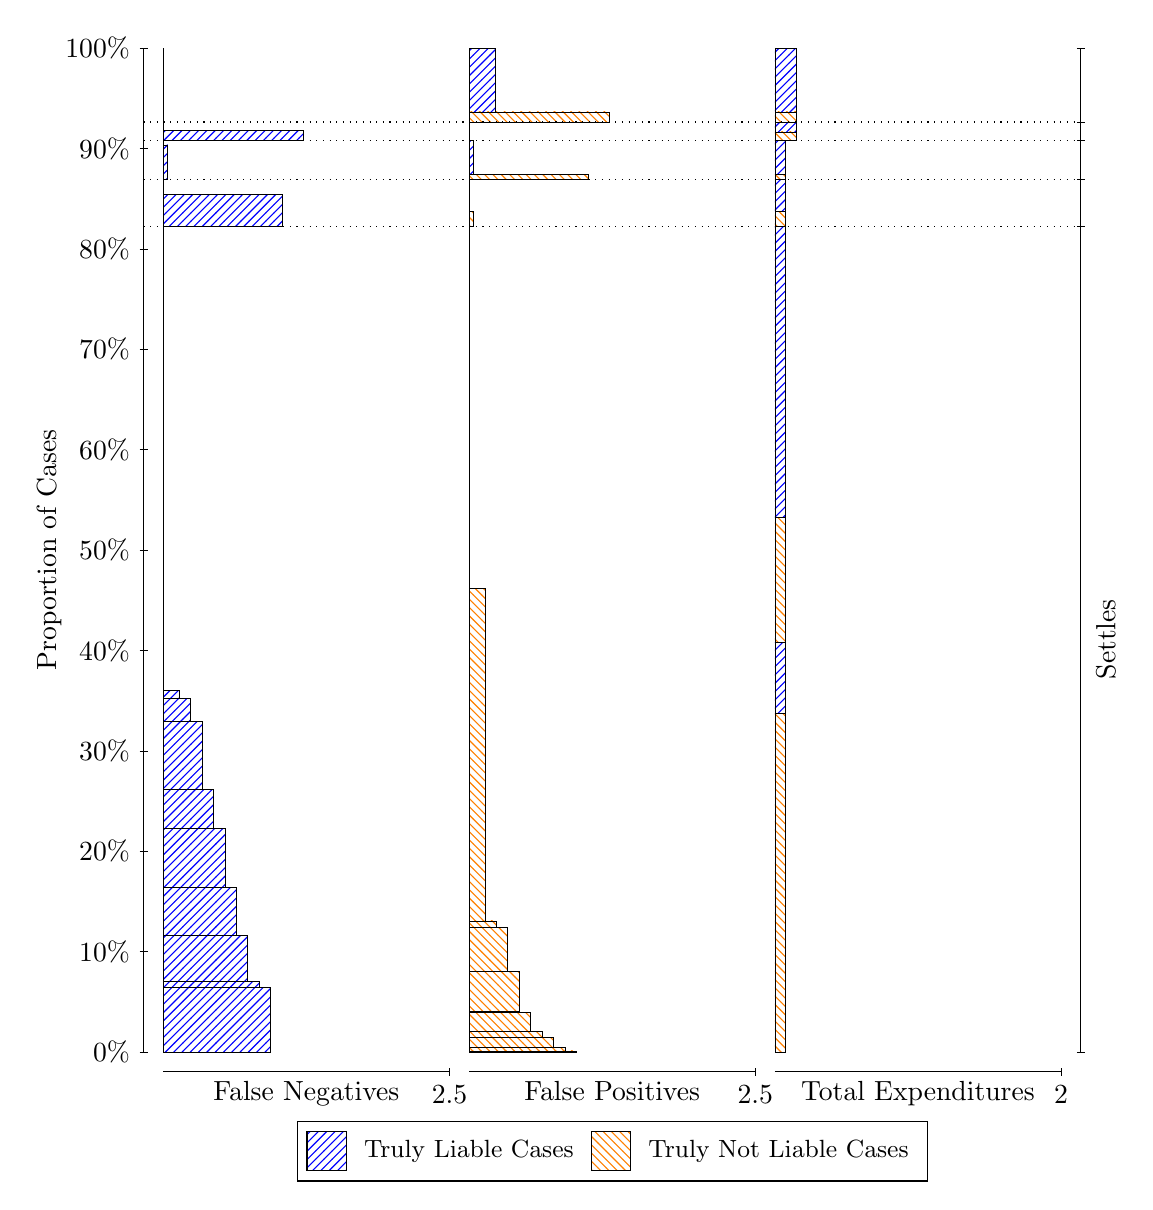
\begin{tikzpicture}
\draw[black, very thin] (1.5,1.75) -- (1.5,14.5);
\node[rotate=90, text=black, anchor=center] at (0.3, 8.125) {Proportion of Cases};
\draw[black, very thin] (1.45,1.75) -- (1.55,1.75);
\node[text=black, anchor=east] at (1.45, 1.75) {0\%};
\draw[black, very thin] (1.45,3.025) -- (1.55,3.025);
\node[text=black, anchor=east] at (1.45, 3.025) {10\%};
\draw[black, very thin] (1.45,4.3) -- (1.55,4.3);
\node[text=black, anchor=east] at (1.45, 4.3) {20\%};
\draw[black, very thin] (1.45,5.575) -- (1.55,5.575);
\node[text=black, anchor=east] at (1.45, 5.575) {30\%};
\draw[black, very thin] (1.45,6.85) -- (1.55,6.85);
\node[text=black, anchor=east] at (1.45, 6.85) {40\%};
\draw[black, very thin] (1.45,8.125) -- (1.55,8.125);
\node[text=black, anchor=east] at (1.45, 8.125) {50\%};
\draw[black, very thin] (1.45,9.4) -- (1.55,9.4);
\node[text=black, anchor=east] at (1.45, 9.4) {60\%};
\draw[black, very thin] (1.45,10.675) -- (1.55,10.675);
\node[text=black, anchor=east] at (1.45, 10.675) {70\%};
\draw[black, very thin] (1.45,11.95) -- (1.55,11.95);
\node[text=black, anchor=east] at (1.45, 11.95) {80\%};
\draw[black, very thin] (1.45,13.225) -- (1.55,13.225);
\node[text=black, anchor=east] at (1.45, 13.225) {90\%};
\draw[black, very thin] (1.45,14.5) -- (1.55,14.5);
\node[text=black, anchor=east] at (1.45, 14.5) {100\%};

\draw[black, very thin] (13.4,1.75) -- (13.4,14.5);
\draw[black, very thin] (13.35,1.75) -- (13.45,1.75);
\node[anchor=west] at (13.35, 1.75) {};
\draw[black, very thin] (13.35,12.233) -- (13.45,12.233);
\node[anchor=west] at (13.35, 12.233) {};
\draw[black, very thin] (13.35,12.836) -- (13.45,12.836);
\node[anchor=west] at (13.35, 12.836) {};
\draw[black, very thin] (13.35,13.327) -- (13.45,13.327);
\node[anchor=west] at (13.35, 13.327) {};
\draw[black, very thin] (13.35,13.56) -- (13.45,13.56);
\node[anchor=west] at (13.35, 13.56) {};
\draw[black, very thin] (13.35,14.5) -- (13.45,14.5);
\node[anchor=west] at (13.35, 14.5) {};

\draw[black, very thin, pattern color=blue, pattern=north east lines] (1.75,1.75) rectangle (3.1125,2.5689);
\draw[black, very thin, pattern color=blue, pattern=north east lines] (1.75,2.5689) rectangle (2.9672,2.6499);
\draw[black, very thin, pattern color=blue, pattern=north east lines] (1.75,2.6499) rectangle (2.8218,3.2345);
\draw[black, very thin, pattern color=blue, pattern=north east lines] (1.75,3.2345) rectangle (2.6765,3.8378);
\draw[black, very thin, pattern color=blue, pattern=north east lines] (1.75,3.8378) rectangle (2.5312,4.5853);
\draw[black, very thin, pattern color=blue, pattern=north east lines] (1.75,4.5853) rectangle (2.3858,5.0894);
\draw[black, very thin, pattern color=blue, pattern=north east lines] (1.75,5.0894) rectangle (2.2405,5.9436);
\draw[black, very thin, pattern color=blue, pattern=north east lines] (1.75,5.9436) rectangle (2.0952,6.2432);
\draw[black, very thin, pattern color=blue, pattern=north east lines] (1.75,6.2432) rectangle (1.9498,6.3469);
\draw[black, very thin, pattern color=orange, pattern=north west lines] (1.75,6.3469) rectangle (1.75,12.233);
\draw[black, very thin, pattern color=blue, pattern=north east lines] (1.75,12.233) rectangle (3.2578,12.64);
\draw[black, very thin, pattern color=orange, pattern=north west lines] (1.75,12.64) rectangle (1.75,12.836);
\draw[black, very thin, pattern color=blue, pattern=north east lines] (1.75,12.836) rectangle (1.8045,13.271);
\draw[black, very thin, pattern color=orange, pattern=north west lines] (1.75,13.271) rectangle (1.75,13.327);
\draw[black, very thin, pattern color=blue, pattern=north east lines] (1.75,13.327) rectangle (3.5303,13.453);
\draw[black, very thin, pattern color=orange, pattern=north west lines] (1.75,13.453) rectangle (1.75,13.56);
\draw[black, very thin, pattern color=orange, pattern=north west lines] (1.75,13.56) rectangle (1.75,13.69);
\draw[black, very thin, pattern color=blue, pattern=north east lines] (1.75,13.69) rectangle (1.75,14.5);
\draw[black, very thin, pattern color=orange, pattern=north west lines] (5.6333,1.75) rectangle (6.9958,1.763);
\draw[black, very thin, pattern color=orange, pattern=north west lines] (5.6333,1.763) rectangle (6.8505,1.8037);
\draw[black, very thin, pattern color=orange, pattern=north west lines] (5.6333,1.8037) rectangle (6.7052,1.9334);
\draw[black, very thin, pattern color=orange, pattern=north west lines] (5.6333,1.9334) rectangle (6.5598,2.0098);
\draw[black, very thin, pattern color=orange, pattern=north west lines] (5.6333,2.0098) rectangle (6.4145,2.2574);
\draw[black, very thin, pattern color=orange, pattern=north west lines] (5.6333,2.2574) rectangle (6.2692,2.2659);
\draw[black, very thin, pattern color=orange, pattern=north west lines] (5.6333,2.2659) rectangle (6.2692,2.775);
\draw[black, very thin, pattern color=orange, pattern=north west lines] (5.6333,2.775) rectangle (6.1238,3.3371);
\draw[black, very thin, pattern color=orange, pattern=north west lines] (5.6333,3.3371) rectangle (5.9785,3.4162);
\draw[black, very thin, pattern color=orange, pattern=north west lines] (5.6333,3.4162) rectangle (5.8332,7.6365);
\draw[black, very thin, pattern color=blue, pattern=north east lines] (5.6333,7.6365) rectangle (5.6333,12.233);
\draw[black, very thin, pattern color=orange, pattern=north west lines] (5.6333,12.233) rectangle (5.6878,12.429);
\draw[black, very thin, pattern color=blue, pattern=north east lines] (5.6333,12.429) rectangle (5.6333,12.836);
\draw[black, very thin, pattern color=orange, pattern=north west lines] (5.6333,12.836) rectangle (7.1412,12.892);
\draw[black, very thin, pattern color=blue, pattern=north east lines] (5.6333,12.892) rectangle (5.6878,13.327);
\draw[black, very thin, pattern color=orange, pattern=north west lines] (5.6333,13.327) rectangle (5.6333,13.434);
\draw[black, very thin, pattern color=blue, pattern=north east lines] (5.6333,13.434) rectangle (5.6333,13.56);
\draw[black, very thin, pattern color=orange, pattern=north west lines] (5.6333,13.56) rectangle (7.4137,13.69);
\draw[black, very thin, pattern color=blue, pattern=north east lines] (5.6333,13.69) rectangle (5.9603,14.5);
\draw[black, very thin, pattern color=orange, pattern=north west lines] (9.5167,1.75) rectangle (9.6529,6.0494);
\draw[black, very thin, pattern color=blue, pattern=north east lines] (9.5167,6.0494) rectangle (9.6529,6.9493);
\draw[black, very thin, pattern color=orange, pattern=north west lines] (9.5167,6.9493) rectangle (9.6529,8.5363);
\draw[black, very thin, pattern color=blue, pattern=north east lines] (9.5167,8.5363) rectangle (9.6529,12.233);
\draw[black, very thin, pattern color=orange, pattern=north west lines] (9.5167,12.233) rectangle (9.6529,12.429);
\draw[black, very thin, pattern color=blue, pattern=north east lines] (9.5167,12.429) rectangle (9.6529,12.836);
\draw[black, very thin, pattern color=orange, pattern=north west lines] (9.5167,12.836) rectangle (9.6529,12.892);
\draw[black, very thin, pattern color=blue, pattern=north east lines] (9.5167,12.892) rectangle (9.6529,13.327);
\draw[black, very thin, pattern color=orange, pattern=north west lines] (9.5167,13.327) rectangle (9.7892,13.434);
\draw[black, very thin, pattern color=blue, pattern=north east lines] (9.5167,13.434) rectangle (9.7892,13.56);
\draw[black, very thin, pattern color=orange, pattern=north west lines] (9.5167,13.56) rectangle (9.7892,13.69);
\draw[black, very thin, pattern color=blue, pattern=north east lines] (9.5167,13.69) rectangle (9.7892,14.5);
\draw[black, dotted] (1.5,12.233) -- (13.4,12.233);
\draw[black, dotted] (1.5,12.836) -- (13.4,12.836);
\draw[black, dotted] (1.5,13.327) -- (13.4,13.327);
\draw[black, dotted] (1.5,13.56) -- (13.4,13.56);
\draw[black, very thin] (1.75,1.5) -- (5.3833,1.5);
\node[text=black, anchor=north] at (3.5667, 1.5) {False Negatives};
\draw[black, very thin] (5.3833,1.45) -- (5.3833,1.55);
\node[text=black, anchor=north] at (5.3833, 1.45) {2.5};

\draw[black, very thin] (5.6333,1.5) -- (9.2667,1.5);
\node[text=black, anchor=north] at (7.45, 1.5) {False Positives};
\draw[black, very thin] (9.2667,1.45) -- (9.2667,1.55);
\node[text=black, anchor=north] at (9.2667, 1.45) {2.5};

\draw[black, very thin] (9.5167,1.5) -- (13.15,1.5);
\node[text=black, anchor=north] at (11.333, 1.5) {Total Expenditures};
\draw[black, very thin] (13.15,1.45) -- (13.15,1.55);
\node[text=black, anchor=north] at (13.15, 1.45) {2};

\node[text=black, centered, rotate=90] at (13.72, 6.9917) {Settles};





\draw (7.449999999999999,1.5) node[draw=none] (baseCoordinate) {};
\begin{scope}[align=center]
        \matrix[scale=0.5, draw=black, below=0.5cm of baseCoordinate, nodes={draw}, column sep=0.1cm]{
            \node[rectangle, draw, minimum width=0.5cm, minimum height=0.5cm, pattern color=blue, pattern=north east lines] {}; &
            \node[draw=none, font=\small, text=black] (B) {Truly Liable Cases}; &
            \node[rectangle, draw, minimum width=0.5cm, minimum height=0.5cm, pattern color=orange, pattern=north west lines] {}; &
            \node[draw=none, font=\small, text=black] (B) {Truly Not Liable Cases}; \\
            };
\end{scope}

\end{tikzpicture}
\end{document}